\documentclass[a4paper,10pt]{article}
\usepackage{luatexja}
\usepackage{luatexja-fontspec}
\usepackage{geometry}
\usepackage{multicol}
\usepackage{titlesec}
\usepackage{setspace}
\usepackage{graphicx}
\usepackage{caption}
\usepackage{indentfirst}
\usepackage{float} % 図の位置を制御するために追加
\usepackage[utf8]{inputenc}
\usepackage{listings}
\usepackage{xcolor}

\geometry{margin=1in}

% 図のキャプションの表記を「図1」のように日本語化
\renewcommand{\figurename}{図}
\captionsetup[figure]{labelformat=default,labelsep=period}


\renewcommand{\tablename}{表}
\captionsetup[table]{labelformat=default,labelsep=period}

\geometry{margin=25mm}
\setstretch{1.2}
\parindent=1em

\titleformat{\section}{\large\bfseries}{\thesection.}{1em}{}

\definecolor{keywordcolor}{rgb}{0.26, 0.38, 0.68}
\definecolor{commentcolor}{rgb}{0.3, 0.6, 0.3}
\definecolor{stringcolor}{rgb}{0.7, 0.2, 0.2}

\lstdefinelanguage{SystemVerilog}{
  morekeywords={module,endmodule,input,output,logic,always_ff,if,else,begin,end,posedge,negedge},
  sensitive=true,
  morecomment=[l]{//},
  morecomment=[s]{/*}{*/},
  morestring=[b]",
}

\lstset{
  language=SystemVerilog,
  basicstyle=\ttfamily\small,
  keywordstyle=\color{keywordcolor}\bfseries,
  commentstyle=\color{commentcolor}\itshape,
  stringstyle=\color{stringcolor},
  numbers=left,
  numberstyle=\tiny,
  stepnumber=1,
  numbersep=5pt,
  frame=single,
  tabsize=2,
  showstringspaces=false,
  breaklines=true,
  breakatwhitespace=true
}

\title{SystemVerilog Code with Listings}

\begin{document}

% タイトルブロック
\begin{center}
\noindent
{\LARGE 第2回輪講資料} \\
{\large 4321 野秋 琳太郎} \\
2025年 6月 27日
\end{center}

\begin{flushright}
指導教員 宮田 尚起
\end{flushright}

% 二段組開始
\begin{multicols}{2}

\section{はじめに}
LEDで光通信をして,「糸なし糸電話」をやりたい.

\section{班の進捗}
全体の進捗は図\ref{fig:block}のとおりである.
今週で,デジタル信号による通信で必要な要素が一通り揃ったことになる.

\begin{figure}[H] % [H]で強制的にここに図を表示
  \centering
  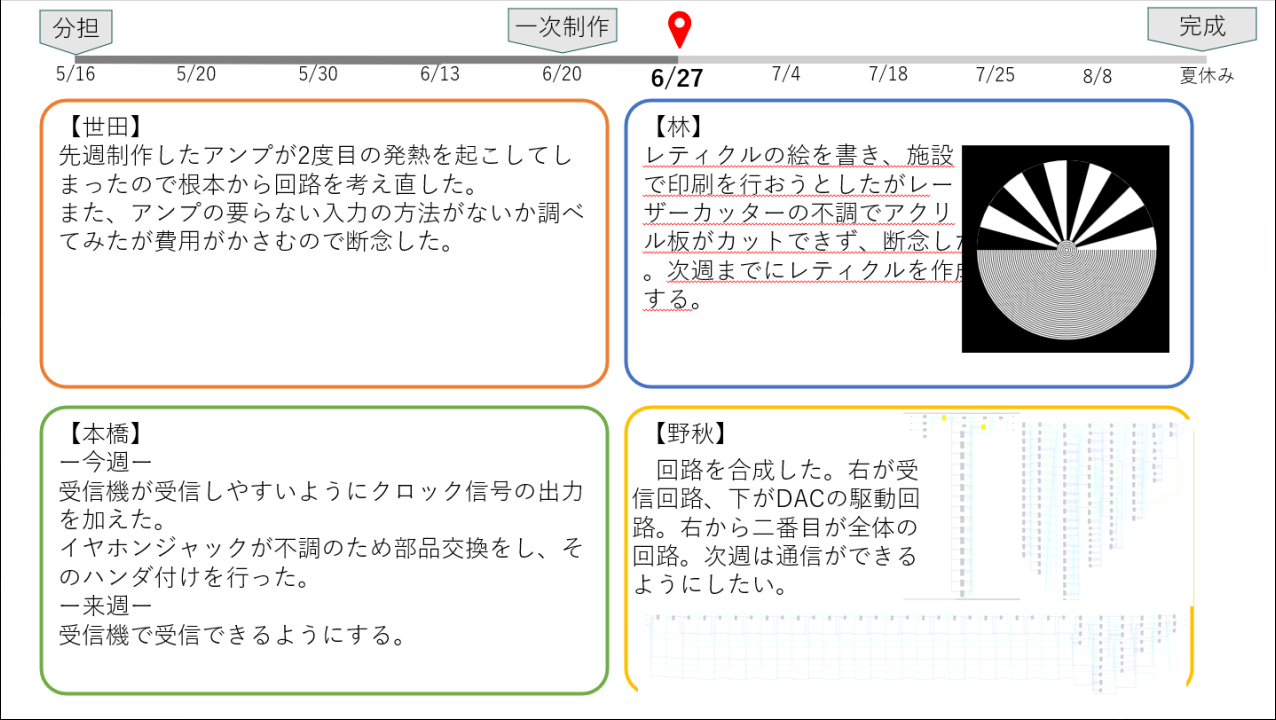
\includegraphics[width=\linewidth]{sintyoku.png}
  \caption{全体の進捗}
  \label{fig:block}
\end{figure}

\section{野秋の進捗}
受信側で使用するFPGAの回路をすべて書いた.
回路は図\ref{fig:system}に示すような構成になっている.

Uartモジュールが受け取る通信のプロトコルは図\ref{fig:uart}のとおりである.
これはuartを16bitに拡張したものであり,データは最上位ビットから順に送られる.

論理合成の結果を表1に示す.
表より,fpgaの容量には余裕があることが分かる.


\begin{figure}[H] % [H]で強制的にここに図を表示
  \centering
  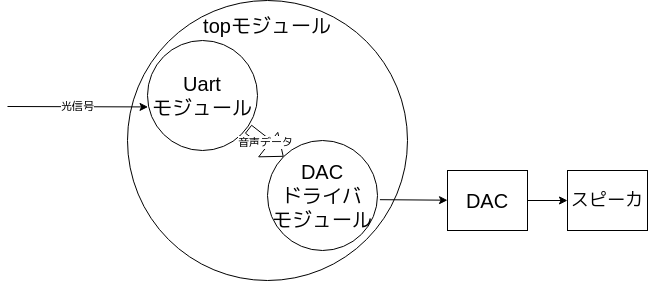
\includegraphics[width=\linewidth]{system.drawio.png}
  \caption{回路のブロック図}
  \label{fig:system}
\end{figure}

\begin{figure}[H] % [H]で強制的にここに図を表示
  \centering
  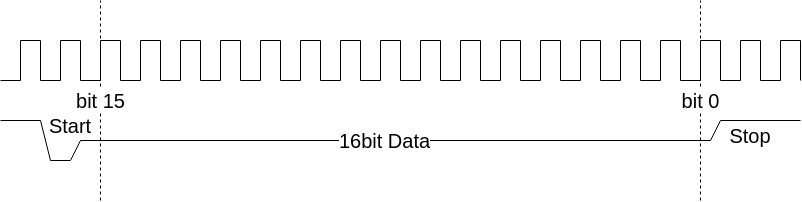
\includegraphics[width=\linewidth]{uart.drawio.png}
  \caption{使用する通信のプロトコル}
  \label{fig:uart}
\end{figure}

\section{今後の予定}
現状,送信したデータを図\ref{fig:hakei}のように反転して受信していた.
これはFPGAで受信したデータを反転させることで対応したい.
\end{multicols}

\begin{table}[H]
\centering
\caption{合成のレポート}
\label{tab:gouesi}
\begin{tabular}{lll}
  \hline
  Resource Utilization Summary &                           &                \\
  \hline
Resource                     & Usage                     & Utilization    \\
Logic                        & 97(93 LUT, 4 ALU) / 20736 & \textless{}1\% \\
Register                     & 97 / 16173                & \textless{}1\% \\
--Register as Latch          & 0 / 16173                 & 0\%            \\
--Register as FF             & 97 / 16173                & \textless{}1\% \\
  BSRAM                        & 0 / 46                    & 0\%          \\
  \hline
\end{tabular}
\end{table}

\begin{figure}[H] % [H]で強制的にここに図を表示
  \centering
  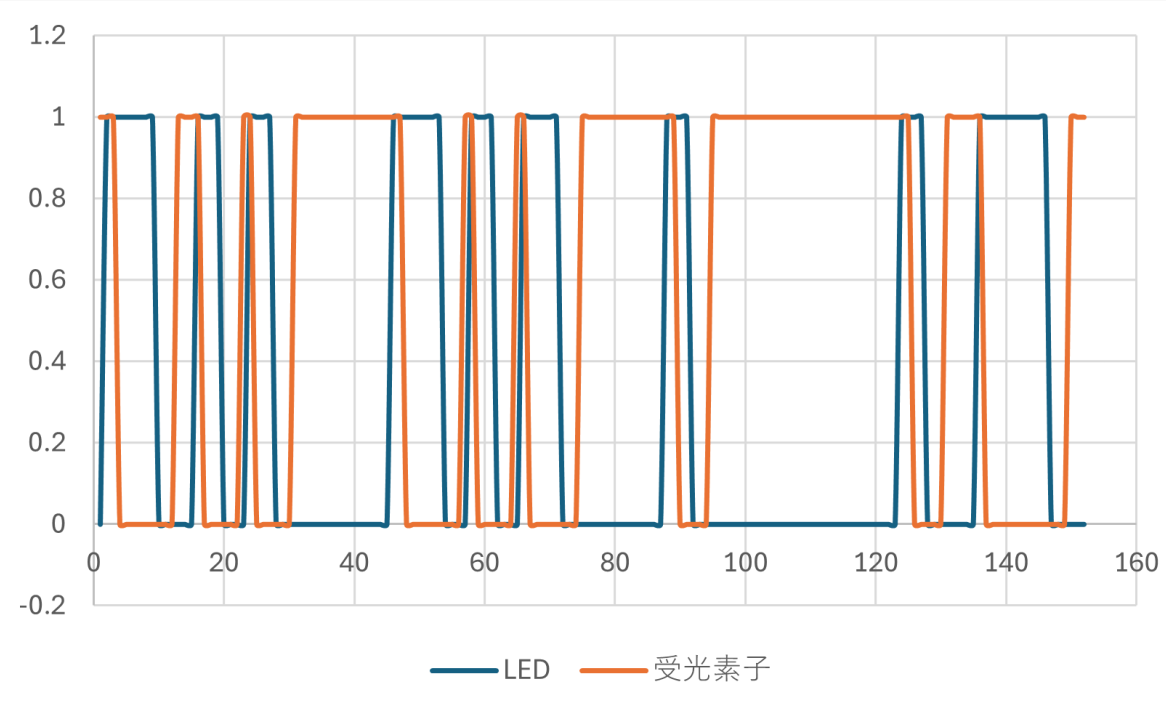
\includegraphics[width=\linewidth]{hakei.png}
  \caption{LEDにかけた電圧と,受光素子で受信した電圧}
  \label{fig:hakei}
\end{figure}

\begin{figure}[H] % [H]で強制的にここに図を表示
  \centering
  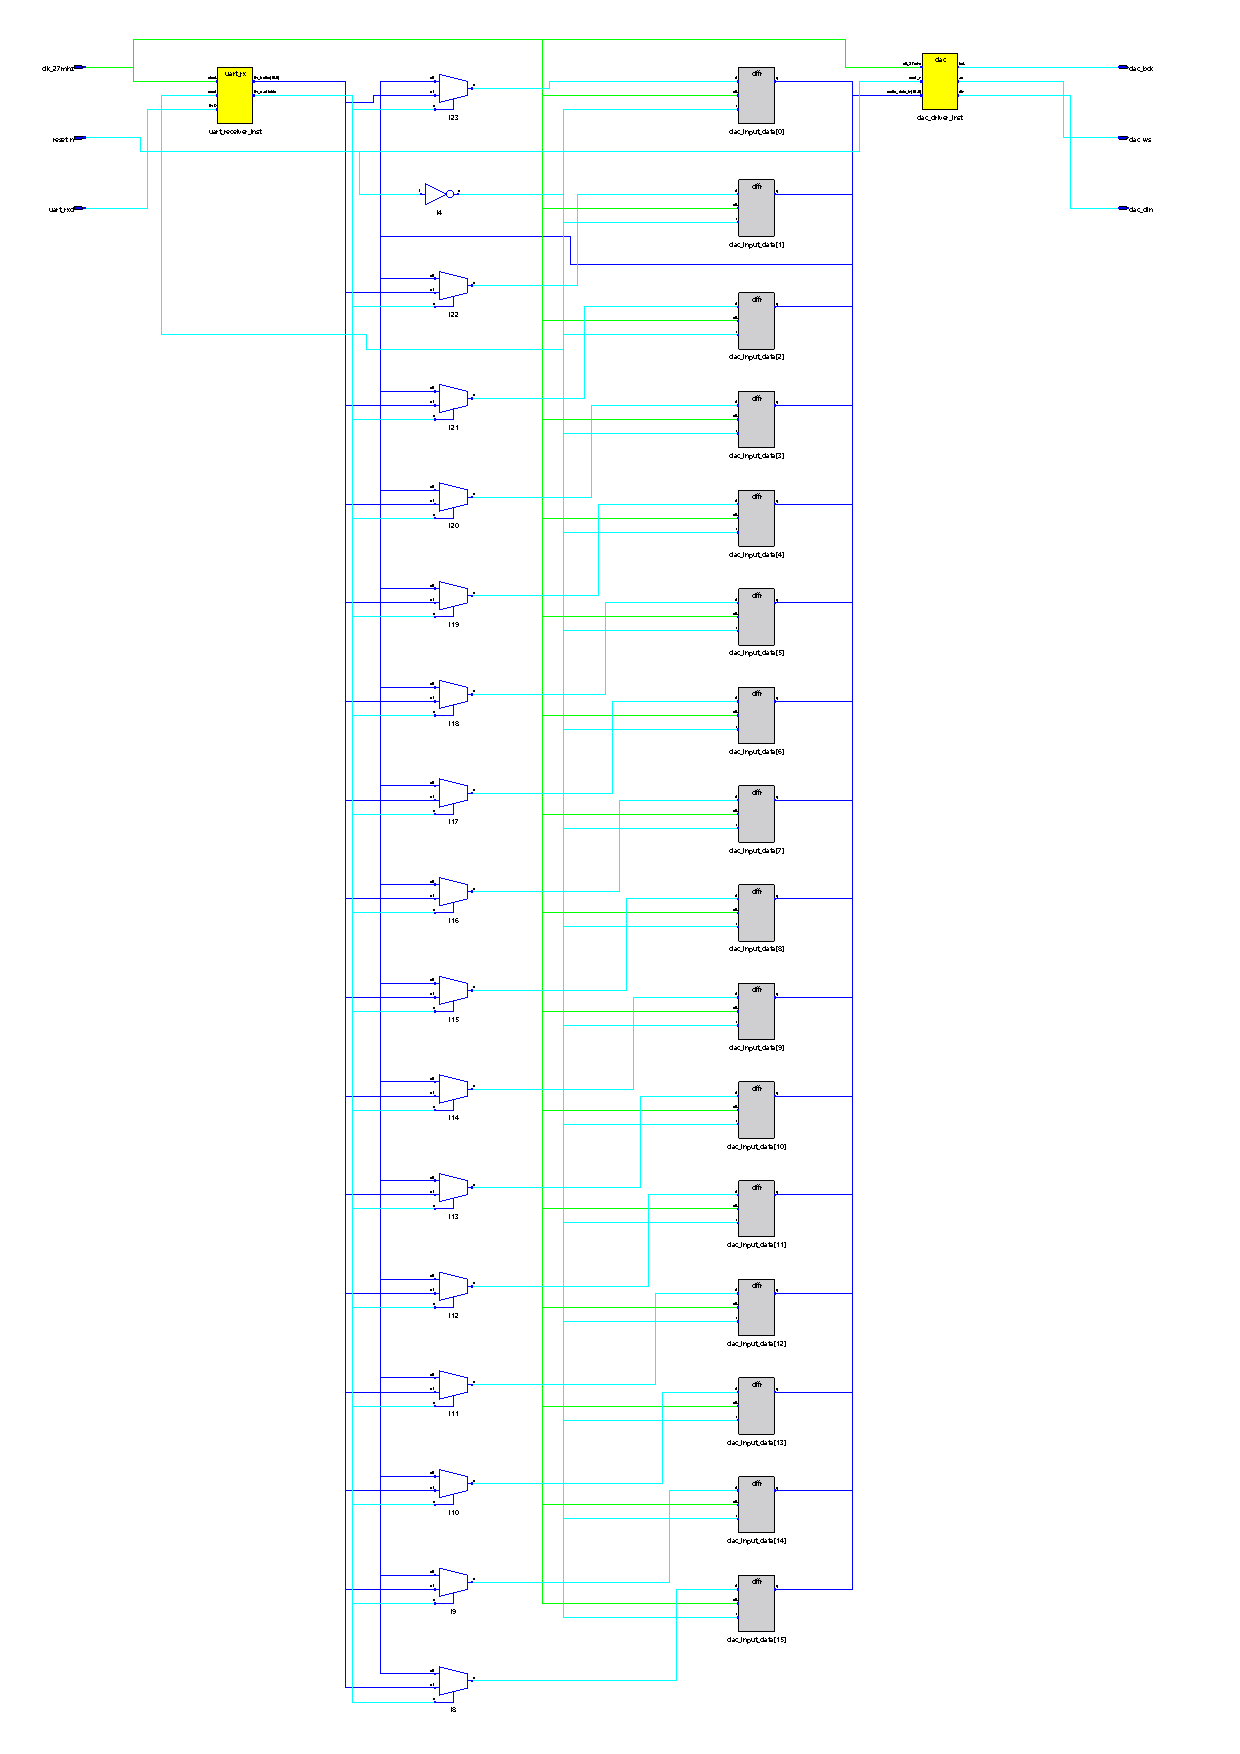
\includegraphics[width=\linewidth]{top.pdf}
  \caption{合成したtopモジュール}
  \label{fig:top_module}
\end{figure}

\begin{figure}[H] % [H]で強制的にここに図を表示
  \centering
  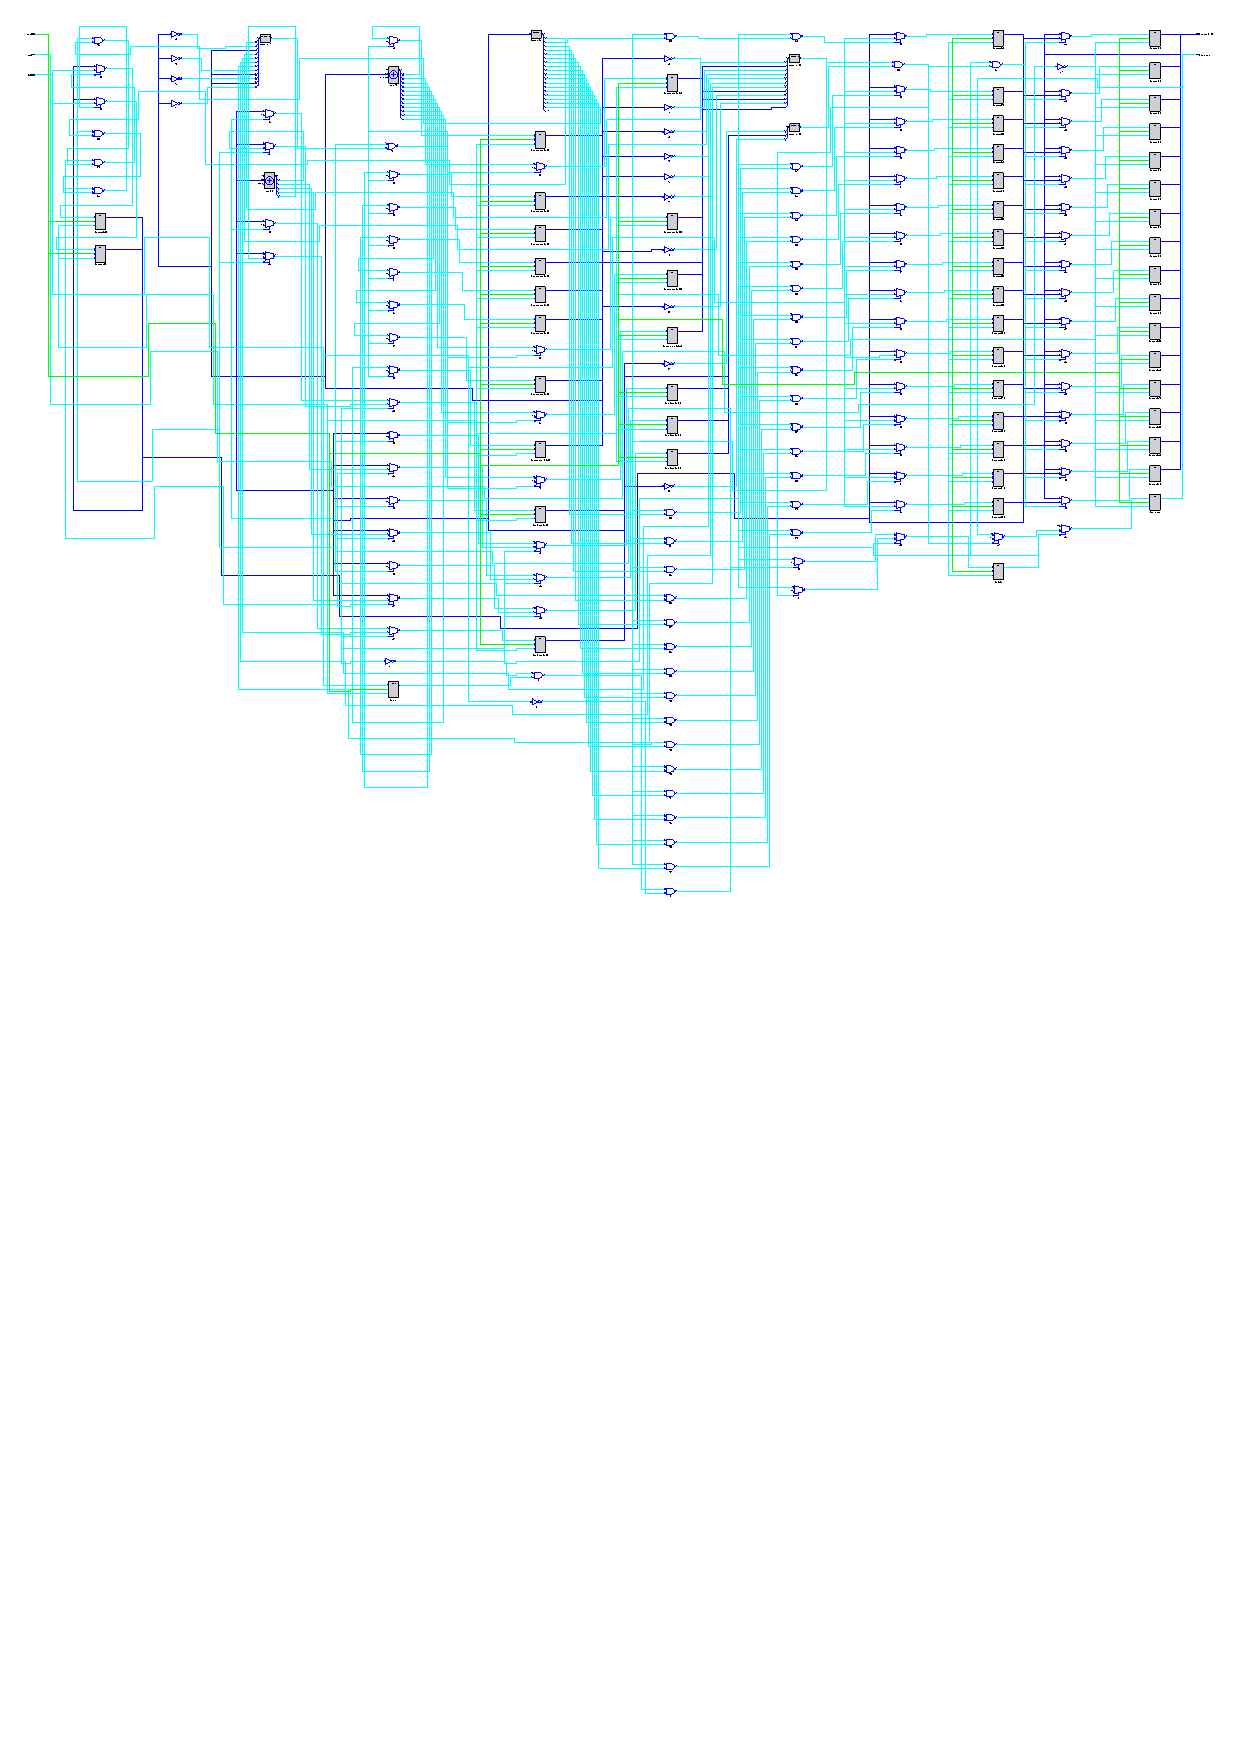
\includegraphics[width=\linewidth]{uart.pdf}
  \caption{合成したuartモジュール}
  \label{fig:uart_module}
\end{figure}

\begin{figure}[H] % [H]で強制的にここに図を表示
  \centering
  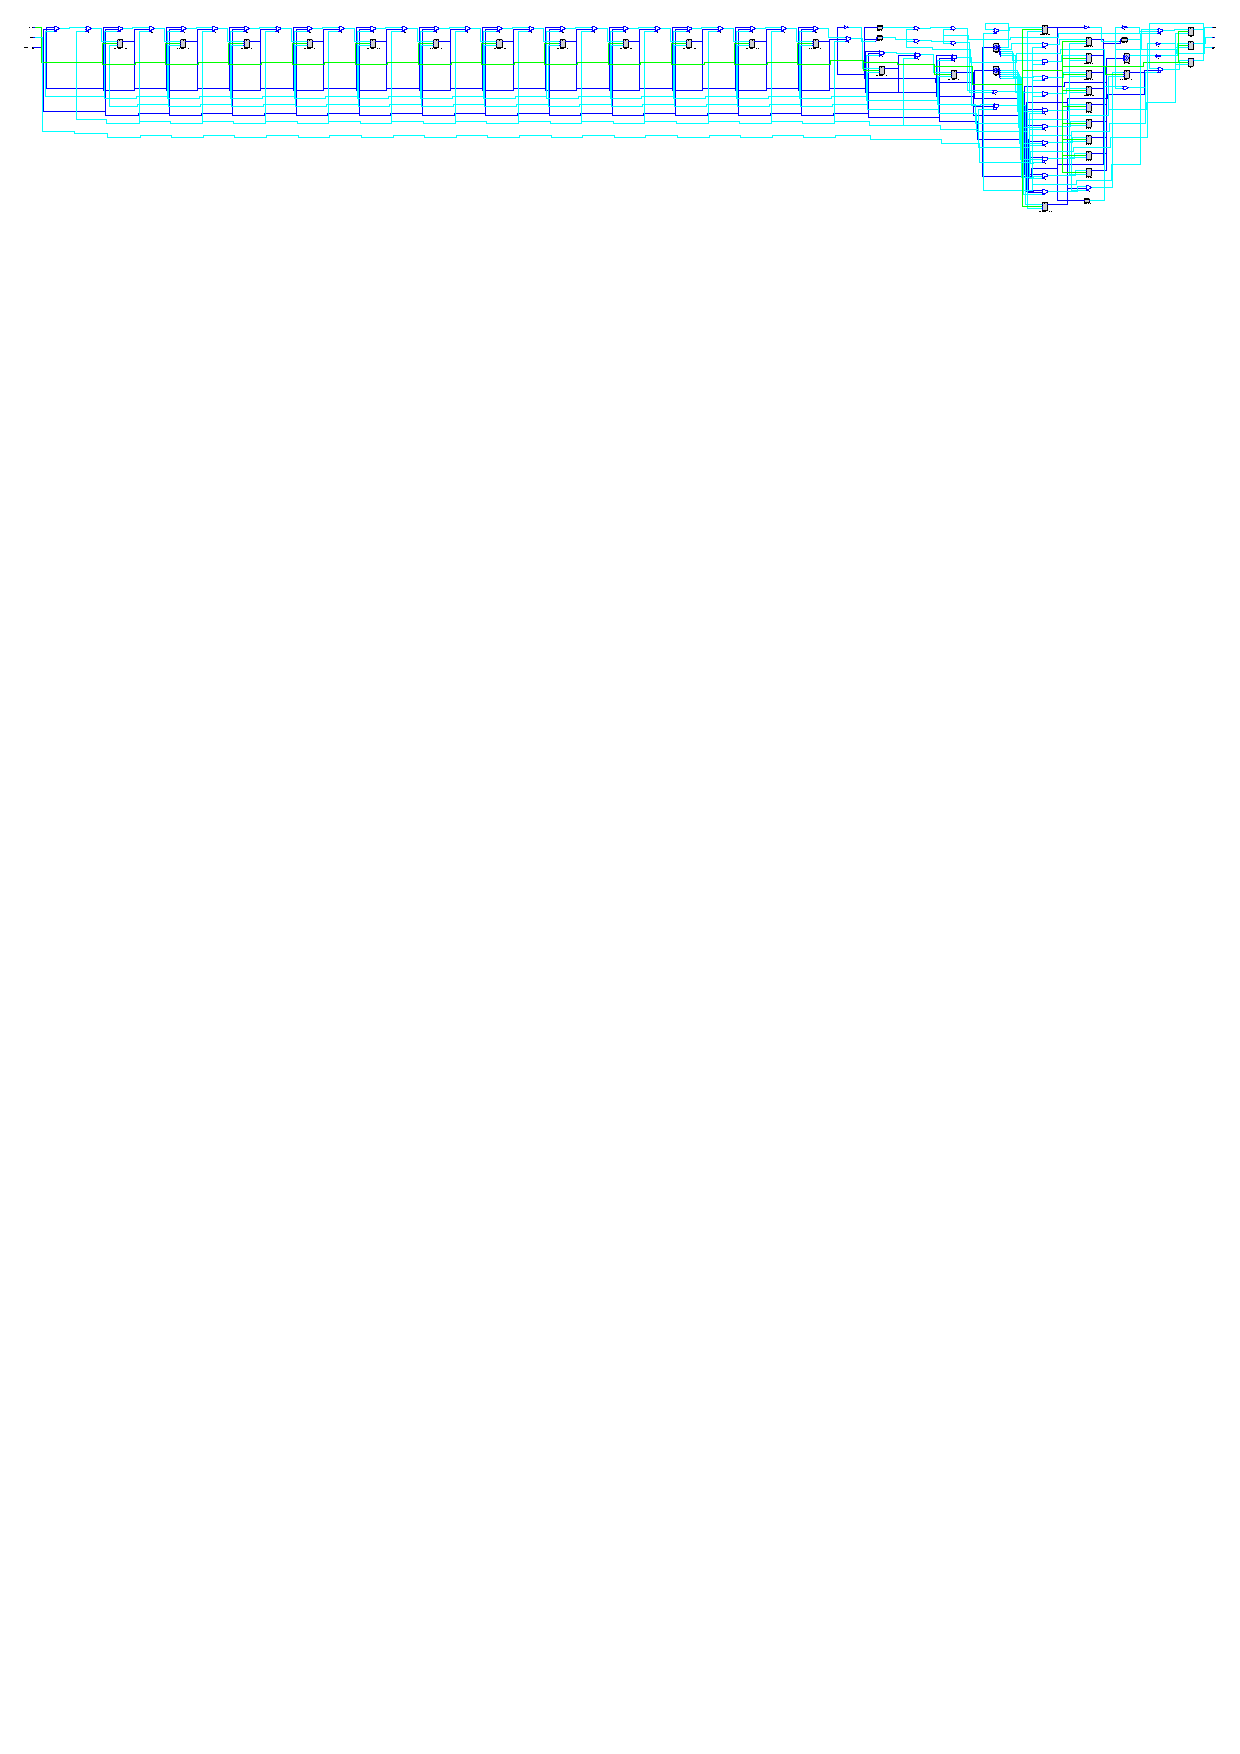
\includegraphics[width=\linewidth]{dac.pdf}
  \caption{合成したdacモジュール}
  \label{fig:dac_module}
\end{figure}

\newpage
\section{書いた回路たち}
\lstinputlisting[caption=topモジュール, label={lst:main}]{src/main.sv}
\newpage
\lstinputlisting[caption=uartモジュール, label={lst:uart}]{src/uart_rx.sv}
\newpage
\lstinputlisting[caption=dacモジュール, label={lst:dac}]{src/dac.sv}
\newpage
\lstinputlisting[caption=IOの割当, label={lst:cst}]{src/miyata_tusin.cst}

\end{document}
